\begin{figure*}[t]
    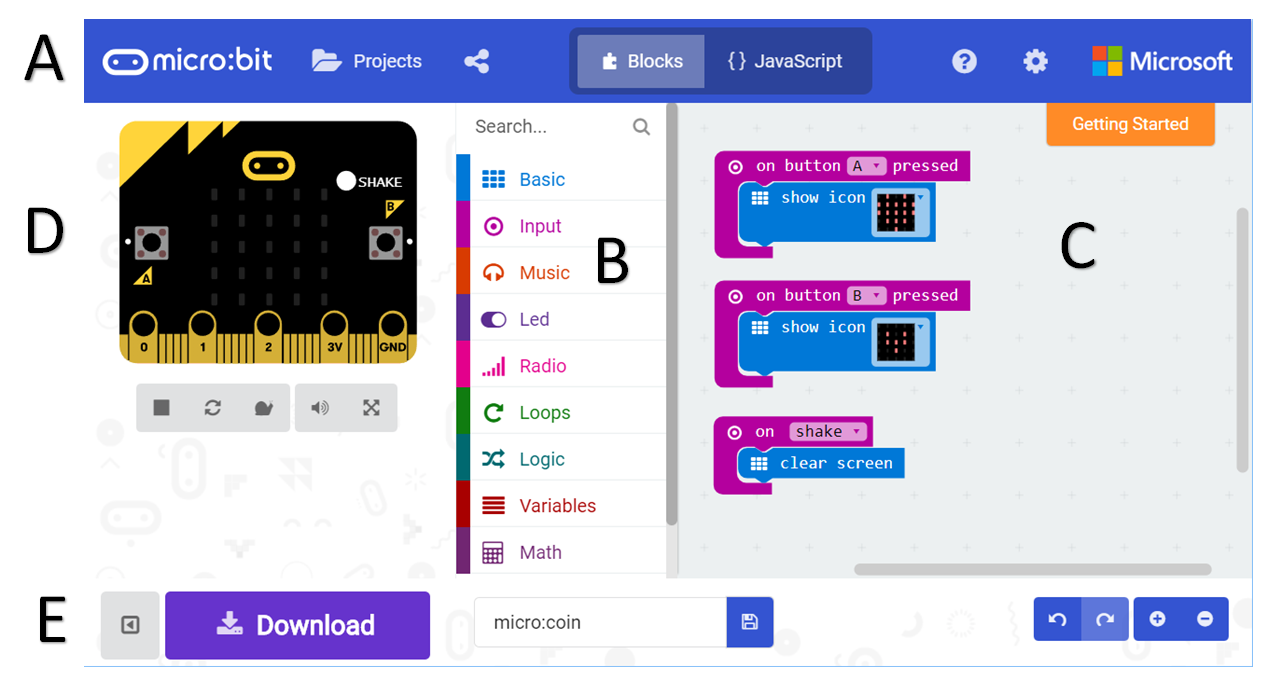
\includegraphics[width=6in]{images/webApp.png}
    \caption{\label{fig:snapshot}MakeCode web app for the micro:bit (\url{http://makecode.microbit.org}).}
  \end{figure*}

\section{The BBC micro:bit}
\label{sec:microbit}
% Talk about the motivations, make people care, provide concrete deliverables

The goals for the BBC micro:bit project were:
\begin{itemize}
    \item[B1] to provide a simple creative experience for physical computing, wearable and Internet of Things (IoT) projects;
    \item[B2] to supply a device that can continue to provide learning opportunities as the user's expertise grows.
    \item[B3] to give students an exciting, engaging introduction to coding;
    \item[B4] to stimulate curiosity about how computing technologies can be utilized to solve problems that students identify.
\end{itemize}

It's important to reiterate the context of the project: 
delivering a micro:bit to every one of 
approximately 3/4 million Year 7 (5th grade) students and teachers in the UK, as
well as 1/4 million micro:bit outside of the school setting; this was a very
broad breadth engagement touching every county in the UK.

In the remainder of this section, we describe the hardware and software
of the micro:bit, the project history, and the experience deploying
the micro:bit in the UK. {\bf callout (perhaps a sidebar) design decisions and
lessons learned: we inherited quite a bit (web app, blockly) but differed
(no C++ compiler needed for user code; ARM DAPlink avoids install for programmer)}

\subsection{The hardware}

Figure~\ref{fig:microbit} shows (a) the front and (b) the back of the
micro:bit, which measures 4cm x 5cm. Like the Arduino Uno,~\cite{ArduinoUno}
the micro:bit is a printed circuit board that makes all its components visible.  
The micro:bit is designed to be engaging from the start, 
with streaks of hair (upper left) and a friendly face (upper middle).
The micro:bit board hosts a variety of sensors (temperature, accelerometer, magnetometer,
light level), a 5x5 LED matrix, two user-defined buttons, as well as Bluetooth
Low Energy (BLE) communications.\footnote{The micro:bit has a whopping
16kB of RAM and 256kB of Flash memory, compared to the Uno's 2kB of
RAM and 32kB of Flash}. 
%More importantly, the device embraces these sensors in its design bringing them to the fore, so to expose its users to the future: a world of embedded, Internet enabled devices.

In contrast to the Uno, which has no built-in sensors, the micro:bit
allows many projects to be completed with no additional hardware or wiring.
The micro:bit's BLE capabilities introduces networking to the
picture, and enables streaming of data and command/control operations among the micro:bit,
smartphones, laptops, as well as other micro:bits.
As with Arduino, an ecosystem of micro:bit shields
(hardware peripherals) that accommodate the micro:bit's edge
connector expands its capabilities (\url{http://microbit.org/resellers/}).
Additionally, the holes in micro:bit's edge connector allows additional external sensors 
and actuators to be connected via crocodile clips or banana plugs.

The micro:bit appears as a USB pen drive when plugged into a host computer;
a compiled program can be transferred to the micro:bit by a simple file copy
operation (flashed). The micro:bit then can be embedded in projects
where it runs on battery power.

The unique combination of features supplied by the micro:bit enables a creative,
extensive experience for physical computing (B1, B2). 
%{\bf [TODO: make sure to note the novel contributions of the project, for those
%readers with research hats on...]}

\subsection{The software}

The design of the micro:bit coding tools also was oriented towards a
simple starting experience with room for progression (B3, B4). Based on in-school trials with a micro:bit prototype, the BBC focused on delivering a web app
based on the popular Blockly framework~\cite{Blocky2015} to permit students to
create scripts via drag-and-drop operations in a web browser, and see
the execution of their scripts via a simulator; text-based coding via scripting languages also
was identified as an important feature. As the micro:bit would be incorporated
into standalone projects, it also was essential for the user's program to be stored on the device for future untethered execution via battery power.

%final design put the entire toolchain in web app, without need to invoke C/C++ compiler to
%compile the user's program; ARM DAPlink solution makes micro:bit appear as USB pen drive
%on all operating systems; MicroPython provided second programming solution with entire toolchain
%on the micro:bit!!]

% less techy here

The solution delivered by the BBC's partners evolved from the initial
design to include support for Blockly, JavaScript and Python, all
via web apps.
Figure~\ref{fig:snapshot} shows a screen snapshot of the MakeCode web app
for the micro:bit,
which supports programming via both Blocky and JavaScript.
The web app has five main sections: (A) menu bar with access to projects
and examples, and switching between Blockly and JavaScript editors; (B)
Blockly toolbox of micro:bit API categories; (C) Blockly programming
canvas with a simple reactive program; (D) micro:bit simulator for execution
of the user's program in browser; (E) download button, which invokes the in-browser
compiler/linker to produce a binary executable.

The Python solution for the micro:bit is based on MicroPython (\url{http://micropython.org})
an implementation of Python 3.0 for microcontrollers. It includes
a full Python compiler and runtime that runs on the micro:bit and
supports a read-eval-print loop (REPL) to execute commands sent via
a terminal, as well as to import and run scripts from the Python web app for
the micro:bit (\url{http://python.microbit.org}).

\subsection{End-to-end experience}

We run through a simple coding example for the micro:bit, as shown
in Figure~\ref{fig:snapshot}(C). The event-based program shown there
in the Blockly editor displays a large heart when the
A button is pressed, displays a small heart when button B is pressed,
and clears the display when the user shakes the micro:bit (shake
detection is implemented using the accelerometer). The interactive
micro:bit simulator
(Figure~\ref{fig:snapshot}(D)) allows the user to test that
the program works as expected. In the simulator, the
shake event is fired using a virtual button (white circle labelled
``SHAKE'').

To generate a binary executable for the micro:bit, the user
simply presses the ``Download'' button (Figure~\ref{fig:snapshot}(E)),
which invokes an in-browser compiler tool chain that translates
the Blockly program to JavaScript and then to machine code, linking
the user's compiled code against a pre-compiled
C++ runtime.~\cite{Devine2018} 
This means that no C++ compiler is required for
compiling the user's program into an executable binary
(The same is true of the MicroPython solution for the micro:bit).

As discussed previously, a simple file copy operation installs the
executable binary on the micro:bit, which appears as a USB pen drive
when plugged into the host computer. This ``lowest-common denominator''
programming method works on all modern operating systems 
(Android, Linux, MacOS, ChromeOS, Windows), as they support 
USB pen drives without the need to install device drivers. 

\subsection{UK rollout: content and training}

{\bf what other stories, data could we bring here }

Great hardware and software do not a full solution make. 
Therefore,
the BBC micro:bit project also called for partners to develop content,
to ``train the trainers'' (educators) around the micro:bit computing
system, and provide hands-on events outside of the school setting to
generate interest in the micro:bit.

As part of the micro:bit project, Clare Riley of Microsoft (Education Relations) directed the curriculum-oriented resource curation and the coordination of training sessions with partners. These were run with Computing At Schools (CAS: a UK non-profit for training educators in CS~\cite{crick2011computing}) ``master'' teachers and operators of extra curricular clubs like UKYouth, Code Club, and CoderDojo. Recipients of the training would be responsible for continuing dissemination at schools and clubs in their vicinity.

% creating a ``cascade effect of teacher training which was really powerful''.

% According to Clare,
% a main challenge of this aspect to the micro:bit project was ``trying to get everybody capable to do it and enthusiastic''; in particular, educators who lack a strong background in computing were ``a bit nervous about all of this, and they are alarmed at the prospect of having to teach computing''. She engaged with a wider group of organisations (UKYouth, Code Clubs, CoderDojo) who had CS background and experience; through training both audiences, each could provide support to the other, offering breadth and support---not only for students, but for the educators as well.

Training consisted of an introductory session with the device and code editors, guiding educators through lesson plans and discussing how the lesson plan met the criteria of the UK curriculum; they were encouraged to play, tweet and blog for the remaining time. Clare noted that the response from her audience to the training sessions was very positive, with a general response of ``100\% wow, let's get going''. She related a story describing the experience of one educator who before commencing training believed that this was ``another rubbish project from people who'd spent too much money the wrong way'', but after engaging with the micro:bit loved it. 

From leveraging the CAS network of teachers, Clare learned that less confident teachers were not comfortable with the single-lesson plan approach of teaching the curriculum. She explained that they ``wanted a 6 or 8 week block of stuff, which said `this is the scheme of work which will deliver these outcomes from the national curriculum''', rather than the individual lessons---they wanted more scaffolding.

Overall, teacher training, combined with the engagement of enthusiastic technologists, alongside structured curriculum-aligned resources were clear contributors to the uptake of the micro:bit in the UK.

\subsection{Project history and open sourcing}

% Previous papers with micro:bit history:

% \begin{itemize}
%     \item \cite{rogers2017bbc} - A brief history of micro:bit, unclear to me if we should include or duplicate.
%     \item \cite{sentance2017creating} - Sue Sentance paper on kids creating stuff with micro:bit
%     \item \cite{knowles2018children} - Lancaster paper on what children want to create using the micro:bit -- inspirational?
% \end{itemize}

As mentioned in the Introduction, the motivation for the BBC micro:bit project
stemmed from the BBC's previous history with computing education via the BBC Micro, 
the desire to address the growing digital divide in the UK~\cite{XYZ},
as well as the UK government's mandate to teach computer science at the K-12 grade levels.

{\bf [Why did the BBC choose physical computing? Need Howard Baker's input on this]}

In 2013-2014 ({\bf CHECK THIS}), the BBC created a prototype of the micro:bit, 
documented via a reference implementation. School trials with this prototype 
informed the BBC's decision to target Year 7. 

In December 2014, the BBC issued an Request for Participation
for ``Delivery of a hands-on learning experience for the Make it Digital season'',
which was the micro:bit project.
The reference implementation and
its design rationale also was made available to the partners to inform
their response.
In the end, 29 partners were invited to contribute hardware, software, services,
teaching materials, packing/distribution, logistics, events and funding.

Work on the project commenced in February 2015, with delivery of
a web site/app in September 2015 (which was critical
for training teachers) and delivery of the micro:bits in the second
half of the 2015-2016 school year.

The BBC micro:bit project partners agreed to open source all assets, both
hardware and software. The main entry points are:
\begin{itemize}
\item \url{https://github.com/bbcmicrobit} for MicroPython, micro:bit hardware design, and micro:bit prototype;
\item \url{https://github.com/microsoft/pxt-microbit} for MakeCode;~\footnote{
MakeCode superceded the TouchDevelop for micro:bit web app~\cite{ball2016microsoft}, also developed by Microsoft.}
\item {\tt \href{https://github.com/lancaster-university/microbit-dal}{microbit-dal}}             for the micro:bit
C++ runtime.
\end{itemize}

